% Dans l'introduction, on présente le problème étudié et les buts
% poursuivis. L'introduction permet de faire connaître le cadre de la
% recherche et d'en préciser le domaine d'application. Elle fournit
% les précisions nécessaires en ce qui concerne le contexte de
% réalisation de la recherche, l'approche envisagée, l'évolution de
% la réalisation. En fait, l'introduction présente au lecteur ce
% qu'il doit savoir pour comprendre la recherche et en connaître la
% portée.
\selectlanguage{french}
\Chapter{INTRODUCTION}\label{sec:Introduction}  % 10-12 lignes pour introduire le sujet.

Même si on ne les voit pas, les satellites artificiels sont essentiels à la société moderne. 
Ils permettent d'acquérir des données scientifiques importantes dans des domaines tels que l'astronomie \cite{Freedman2001}, l'étude des plaques tectoniques et des volcans \cite{Christodoulidis1985}, la climatologie \cite{Hollmann2013}, le suivi de l'état des glaciers \cite{Goldstein1993} ou l'analyse de l'état de l'atmosphère \cite{Laube2014}. 
Également, ils ont de nombreuses applications civiles telles que les prévisions météorologiques \cite{Bauer2015}, la navigation \cite{Getting1993}, les télécommunications \cite{Evans2005}, l'agriculture \cite{Lobell2002} ou la mesure de l'étendue des désastres majeurs \cite{Tralli2005}.  
Qu'ils soient opérés par des entités gouvernementales ou privées, tous les satellites doivent être positionnés en orbite à l'aide de lanceurs de satellites. 
Ces derniers doivent garantir des niveaux de fiabilité très élevés et livrer avec une très grande précision les satellites sur les trajectoires convenues tout en minimisant les couts. 

Le potentiel commercial d'un lanceur de satellite est fortement lié au ratio entre la masse utile qu'il peut élever en orbite et sa masse. 
Afin d'optimiser ce ratio, il est nécessaire de sélectionner des matériaux offrant de bonnes propriétés mécaniques ainsi qu'un poids minimal. 
Les matériaux composites permettent d'atteindre ces deux buts en permettant de créer des pièces aux propriétés optimisées en fonction de l'application, et ce, tout en minimisant leur masse. 
Le développement d'une nouvelle génération de lanceurs en matériaux composites est justifié par des impératifs techniques ainsi qu'économiques. 
Cependant, la transition vers les matériaux composites pose de nombreux défis. 

Dans la conception des lanceurs modernes, les réservoirs de carburant et de comburant agissent comme composants structurels et supportent le poids du lanceur et de la charge utile. 
Dans le cas \mbox{d'Ariane 6}, ces réservoirs ainsi que de nombreux composants en matériaux composites seront produits par déposition automatisée de fibres (AFP) ou par enroulement filamentaire avec une consolidation \textit{in situ} au laser \cite{Krzeminski2014}. 
Les jupettes quant à elles agissent comme éléments de transition entre les sections et les étages du lanceur. 
Ainsi, le joint structurel entre une jupette et un réservoir (Fig.~\ref{fig:schema_jonction}) doit supporter les forces rencontrées durant le décollage et est nécessaire au maintien de l'intégrité du lanceur. 
De plus, cette jonction doit être flexible, car, pendant le décollage, le diamètre des réservoirs change en fonction de leur pression interne résiduelle. 
Ces déformations doivent alors être absorbées par les joints avec les jupettes. 
L'emploi de jonctions flexibles permet également d'absorber une partie des vibrations causées lors du décollage et ainsi de minimiser les charges que doit supporter le chargement. 
Dans le cas d'assemblages de pièces en composite, une grande attention doit être portée aux jonctions entre les composants. 
Ces dernières sont généralement des points critiques pour la conception des structures. 
Dans ce cas particulier, la jonction entre la jupette et le réservoir présente des conditions d'opération particulièrement difficiles. 

\begin{figure}[h!]
	\centering
	\subfigure[]
	{\label{fig:schema_jonction_a} 								
		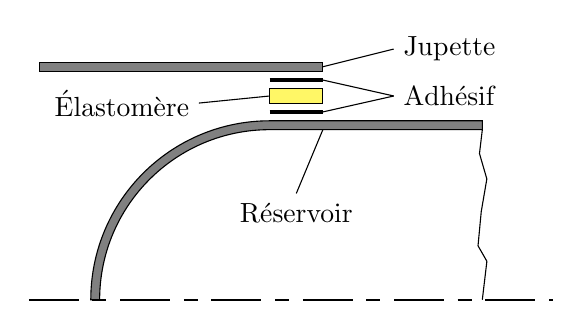
\begin{tikzpicture}[scale=0.9]

%Couleurs
\def \colelastomere{yellow!60}
\def \colreservoir{black!50}

%Dimentions du réservoir et de la jupette
\def \epaisseurreservoir{.125}
\def \ldroit{3}
\def \laxe{1.}
\def \tjupette{0.125}
\def \ljupette{4}
\def \rayonint{0.6*\ljupette}

%Définition de l'espace entre les éléments de la soudure
\def \espace{0.125}
\def \lsoudure{0.75}
\def \telastomere{0.2}

\tikzstyle{loosely dashed}=      [dash pattern=on 18pt off 5pt on 5pt off 5 pt]

%paroi du réservoir
\draw[black,fill=\colreservoir] (0,\rayonint) arc (90:180:\rayonint) -- ++ (- \epaisseurreservoir,0) arc (180:90:\rayonint+\epaisseurreservoir) -- ++ (\ldroit,0) -- ++ (0,-\epaisseurreservoir) -- cycle; 
\draw[black,decorate,decoration=random steps] (\ldroit,\rayonint) -- ++ (0,-\rayonint);

%Axe
\draw[black,thick,loosely dashed] (-\rayonint-\laxe,0) -- ++ (\rayonint+\ldroit+2*\laxe,0);

%Éléments chauffants
\draw[black,very thick] (0,\rayonint+\epaisseurreservoir+\espace) -- ++(\lsoudure,0);
\draw[black,very thick] (0,\rayonint+\epaisseurreservoir+3*\espace+\telastomere) -- ++(\lsoudure,0);

%Élastomère
\draw[black,fill=\colelastomere] (0,\rayonint+\epaisseurreservoir+2*\espace) -- ++(\lsoudure,0) -- ++(0,\telastomere) -- ++ (-\lsoudure,0) -- cycle;

%Jupette
\draw[black,fill=\colreservoir] (\lsoudure,\epaisseurreservoir+4*\espace+\telastomere+\rayonint)  -- ++ (-\ljupette,0) -- ++ (0,\tjupette) -- ++(+\ljupette,0)  -- cycle; 

%Identification
\draw[black,thin] (\lsoudure,\epaisseurreservoir+4*\espace+\telastomere+\rayonint+0.5*\tjupette) -- ++ (1,2*\espace) node[right] {Jupette};

\draw[black,thin] (\lsoudure,\epaisseurreservoir+3*\espace+\telastomere+\rayonint) -- ++ (1,-\espace-0.5*\telastomere) ;

\draw[black,thin] (0,\epaisseurreservoir+2*\espace+0.5*\telastomere+\rayonint) -- ++ (-1,-0.5*\telastomere) node[left] {Élastomère};

\draw[black,thin] (\lsoudure,\epaisseurreservoir+\espace+\rayonint) -- ++ (1,\espace+0.5*\telastomere) node[right] {Adhésif};

\draw[black,thin] (0.25*\ldroit,\rayonint) -- ++ (-0.5*\lsoudure,-0.375*\rayonint) node[below] {Réservoir};

%\node[inner sep=0pt] (SaturnV) at (9,2)
%{\includegraphics[width=.5\textwidth]{SaturnV_stage2.pdf}};
%
%\node (a) at (1,-3) {a)};
%\node (b) at (9,-3) {b)};
%
%\draw[red,very thick] (6.6,1) ellipse [x radius=1.5,y radius=0.4];
%\draw[red,very thick] (6.6,3.9) ellipse [x radius=1.5,y radius=0.4];

\end{tikzpicture}
	} \qquad
	\subfigure[]
	{\label{fig:schema_jonction_b}
		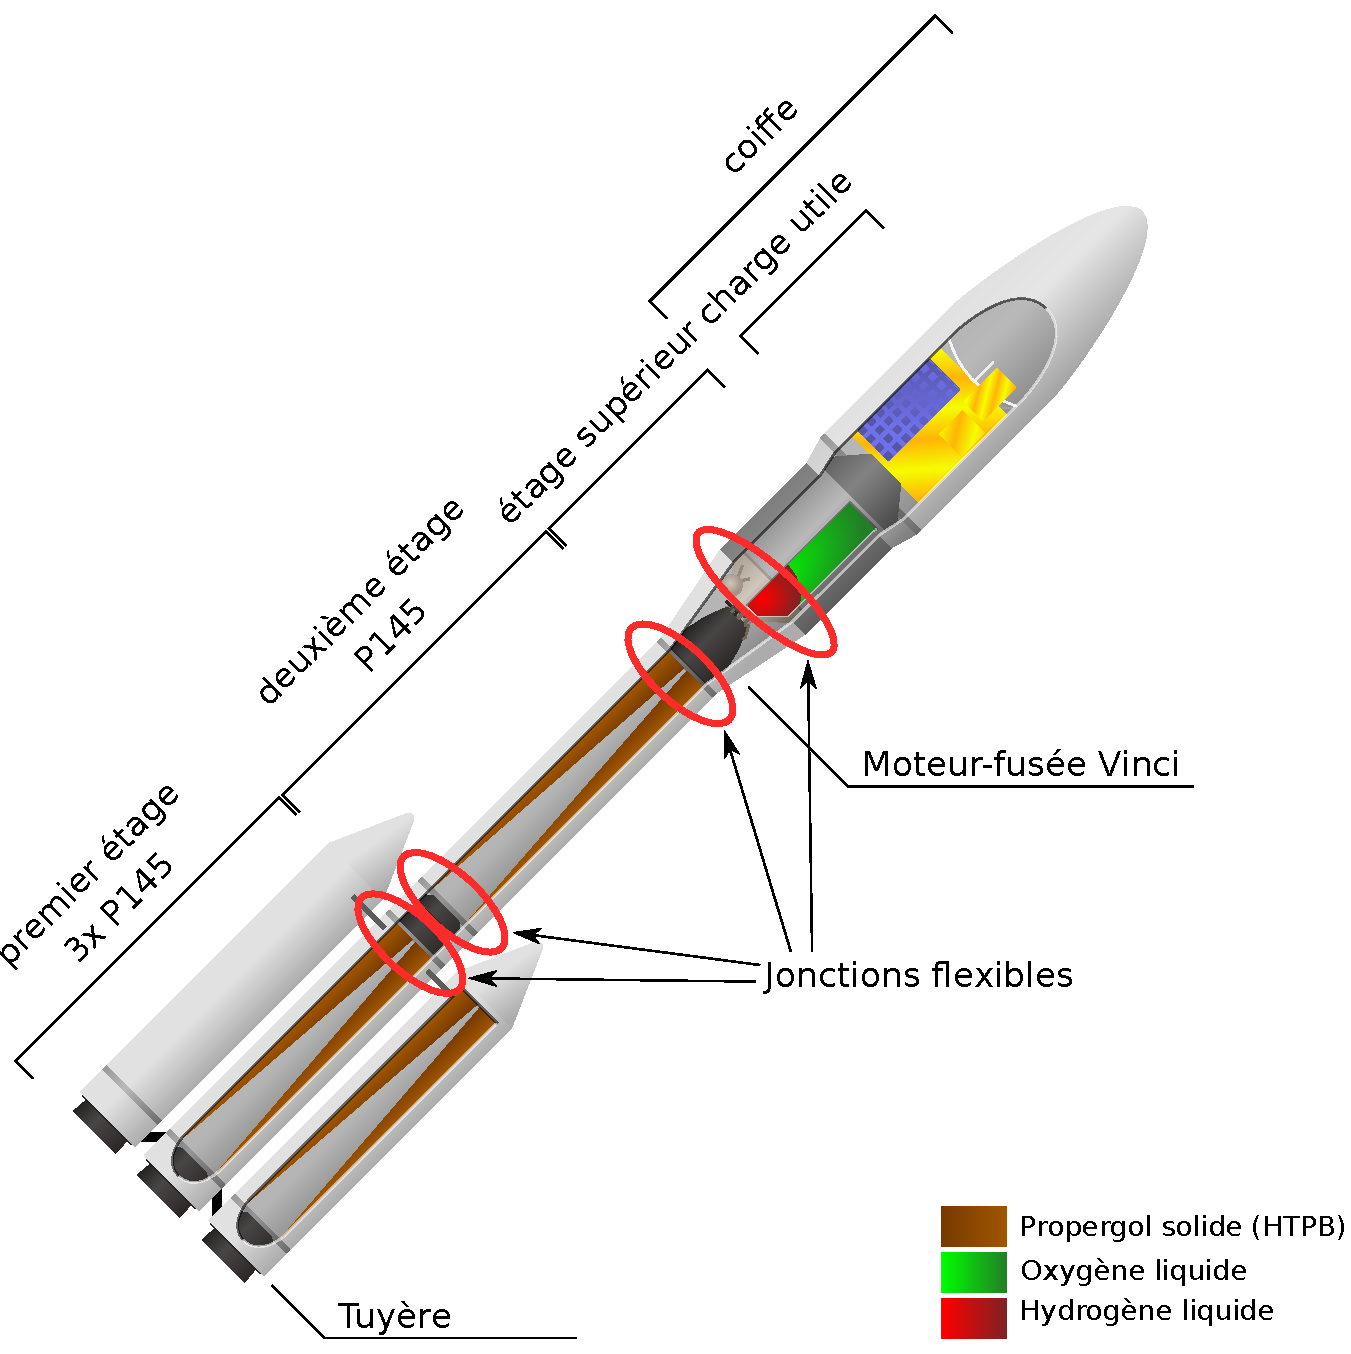
\includegraphics[width=0.45\textwidth]{Ariane_6_PPH_cutaway.pdf}
	}
	\caption{a) Schéma de la jonction flexible entre le réservoir et la jupette, b) emplacement des jonctions sur la fusée Ariane 6 (adaptée de \cite{Wikipedia:Ariane6}, sous licence Creative Commons)}
	\label{fig:schema_jonction}
\end{figure}

Une solution initiale employant des colles structurelles et un élastomère réticulé permettait d'atteindre les requis de performance pour les lanceurs fabriqués en composites thermodurcissables. 
En raison de problèmes de sensibilité environnementale lors de la préparation des joints et de longs temps de mise en œuvre, ArianeGroup a décidé d'explorer la possibilité de passer aux composites à matrice thermoplastique. 
Tout d'abord, cette transition leur permettra d'accélérer les cadences de production et de tirer profit des propriétés des composites à matrice thermoplastique telles que leur plus grande résistance aux impacts et, dans certains cas, aux solvants. 
Ensuite, cette conversion leur permettra d'augmenter la robustesse du joint et d'éviter des problèmes liés au collage tels que de longs temps de réticulation et une grande sensibilité à la préparation des surfaces et aux contaminants. 
Afin de compléter cette transition vers des structures en composites à matrices thermoplastiques, il est nécessaire de développer une nouvelle solution. 

L'objectif général des travaux présentés dans le cadre de cette thèse est de développer un procédé de soudage par résistance utilisant un nanocomposite conducteur comme élément chauffant pour joindre un adhérent en composite thermoplastique et un élastomère thermoplastique. 

%%
%%  CONCEPTS DE BASE / BASIC CONCEPTS
%%
%\section{Concepts de base}


\section{Éléments de la problématique}

La production d'une jonction flexible entre des adhérents en composite thermoplastique nécessite l'obtention de soudures multiples avec des matériaux aux propriétés très différentes. 
Sur le plan des concepts, le processus de soudage s'apparente aux processus de formation des lignes de soudures lors de la fabrication par injection de pièces en polymère ou lors de l'injection subséquente d'un autre polymère pour produire un surmoulage. 

Dans un premier temps, il sera nécessaire d'explorer les concepts associés au soudage tels que l'autohésion et la diffusion des chaines de polymères. 
Une recension des écrits concernant le soudage des composites thermoplastiques permettra de bien cibler les paramètres clés à optimiser et d'établir des comparatifs avec les résultats qui sont obtenus. 

En second lieu, pour la jonction avec l'élastomère, peu de réponses existent déjà dans la littérature scientifique.
Il est donc nécessaire de développer une approche expérimentale progressive et méthodique pour résoudre cette portion du problème. 

%%
%% PLAN DU MEMOIRE / THESIS OUTLINE
%%
\section{Plan de la thèse}  % 0.5 page

À la suite de cette introduction, le chapitre \ref{sec:RevLitt} présentera l'ensemble des connaissances contenues dans les travaux publiés ayant rapport à la production de jonctions flexibles par soudage résistif. 
Cette section discutera tout d'abord des matériaux composites, des techniques de mise en forme ainsi que des paramètres propres au soudage. S'ensuivra une section à propos des nanocomposites conducteurs d'électricité. Le chapitre se terminera avec une courte discussion sur les élastomères thermoplastiques.

Par la suite, au chapitre \ref{sec:Objectifs}, une analyse objective des écrits publiés permettra de cerner les limites de la connaissance actuelle et de définir plus particulièrement les objectifs de recherche. 

Les chapitres \ref{sec:Theme1} à \ref{sec:Theme3} quant à eux présenteront les principaux travaux réalisés dans le cadre de cette thèse. 
Les sujets de ces chapitres seront directement en lien avec les objectifs précédemment présentés. 

Le chapitre \ref{sec:Discussion} traitera de travaux ayant été réalisés dans le cadre de cette thèse, mais ne figurant pas dans les thématiques abordées dans le cadre des travaux principaux présentés aux chapitres \ref{sec:Theme1} à \ref{sec:Theme3}.  

Le chapitre \ref{sec:Contributions} mettra en valeur les contributions originales de ces recherches. 
Ce chapitre présentera une synthèse des principaux résultats positifs et négatifs. 
Il démontrera comment les travaux réalisés durant cette thèse ont permis d'avancer le niveau de connaissance par rapport au soudage par résistance et à la production de jonction flexible. 
Ce chapitre portera également un regard critique sur les résultats obtenus en recherchant les limites d'applicabilité des nouvelles connaissances et se conclura par la suggestion de pistes pour de nouveaux projets de recherche. 
